\documentclass[a4paper, 12pt]{article} % Artikel-Klasse

%---------------------------------------------------------
% Encoding, language, quotes
%---------------------------------------------------------
\usepackage[utf8]{inputenc}
\usepackage[ngerman]{babel}       % Deutsche Sprache und Silbentrennung
\usepackage{csquotes}             % Für korrekte Anführungszeichen
\usepackage{listings}
\usepackage{xcolor}

%---------------------------------------------------------
% Graphics & PDF
%---------------------------------------------------------
\usepackage{graphicx}
\usepackage{pdfpages}             % Einbinden von PDF-Seiten
\usepackage{caption}              % Verbesserte Bildunterschriften
\usepackage{subcaption}

% Customize settings
% Customize settings for a more compact style
\lstset{
    language=Java,                 % Specify Java language for syntax highlighting
    basicstyle=\ttfamily\small,    % Use smaller monospaced font for code
    keywordstyle=\color{blue},     % Style for keywords
    commentstyle=\color{gray},     % Style for comments
    stringstyle=\color{red},       % Style for strings
    numbers=none,                  % No line numbers
    breaklines=true,               % Break long lines
    frame=none,                    % No frame around the code
    xleftmargin=0pt,               % Remove left margin
    xrightmargin=0pt,              % Remove right margin
    aboveskip=5pt,                 % Reduce space above the code block
    belowskip=5pt                  % Reduce space below the code block
}

%---------------------------------------------------------
% Math, units, spacing, etc.
%---------------------------------------------------------
\usepackage{siunitx}
\usepackage{setspace}
\usepackage{textgreek}

% Add float package for "H" float option
\usepackage{float}

%---------------------------------------------------------
% Other packages
%---------------------------------------------------------
\usepackage{ifthen}
\usepackage{acronym}
\PassOptionsToPackage{hyphens}{url} % URLs in Hyperlinks umbrechen
\usepackage[breaklinks=true]{hyperref} 
\usepackage{array}                % Bessere Tabellenformatierung
\usepackage{enumitem}             % Kontrolle über Listen-Layouts
\usepackage{nomencl}
\usepackage{scrlayer-scrpage}     % Header und Footer

% Adjust header and footer heights
\setlength{\headheight}{14.5pt}
\setlength{\footheight}{34.16666pt}

%---------------------------------------------------------
% Bibliography (biblatex mit Biber)
%---------------------------------------------------------
\usepackage[backend=biber, style=ieee]{biblatex}  
\addbibresource{literatur.bib}  

%---------------------------------------------------------
% Platzhalter
%---------------------------------------------------------
\newcommand{\titel}{Verbesserung eines Bluetooth-basierten Warnsystems für den Straßenverkehr durch Datenlogging und innovative Visualisierungstechniken}
\newcommand{\untertitel}{}
\newcommand{\arbeit}{Studienarbeit T3200}
\newcommand{\studiengang}{Elektrotechnik}
\newcommand{\studienrichtung}{Fahrzeugelektronik}
\newcommand{\autor}{Luka Tadic}
\newcommand{\abgabe}{14.07.2025}
\newcommand{\bearbeitungszeitraum}{07.04.2025 - 14.07.2025}
\newcommand{\matrikelnr}{5726700}
\newcommand{\kurs}{TFE22-1}
\newcommand{\firma}{}
\newcommand{\betreuerfirma}{Prof. Dr. Ing. Tobias Frank}
\newcommand{\gutachterdhbw}{Prof. Dr. Ing. Tobias Frank}
\newcommand{\jahr}{2025}

%---------------------------------------------------------
% Header und Footer mit Linien
%---------------------------------------------------------
\clearpairofpagestyles         % Standard-Stile löschen

% Header with consistent logo placement and line position
\ohead{%
    \raisebox{1cm}[0pt][0pt]{% Raise the logo well above the line
        
\includegraphics[width=3cm]{images/DHBW_d_R_FN_46mm_4c}%
    }%
    \\[-1.5cm] % Move the header line down
    \rule{\textwidth}{0.4pt} % Horizontal rule for the header line
}


% Footer with consistent alignment and contents below the line
\setkomafont{pagefoot}{\normalfont} % Ensure consistent font style
\cfoot{%
    \rule{\textwidth}{0.4pt}\\ % Horizontal rule
    \vspace{0.3em} % Small vertical space
    \begin{tabular}{@{}p{0.33\textwidth}p{0.33\textwidth}p{0.33\textwidth}@{}}
        \arbeit & \centering \autor & \raggedleft \thepage
    \end{tabular}
}


\pagestyle{scrheadings}        % Stil aktivieren

%---------------------------------------------------------
% Dokumentbeginn
%---------------------------------------------------------
\begin{document}
\sloppy

%---------------------------------------------------------
% Titelseite
%---------------------------------------------------------
\thispagestyle{empty}  % Kein Header oder Footer auf der Titelseite
\hypersetup{pageanchor=false}

\begin{titlepage}
\enlargethispage{4.0cm}
\sffamily  % Serifenlose Schrift für die Titelseite

\parbox{0.5\linewidth}{
    \begin{flushleft}
        % Optional: Firmenlogo
    \end{flushleft}
}
\parbox{0.5\linewidth}{
    \begin{flushright}
        
\includegraphics[width=0.4\linewidth]{images/DHBW_d_R_FN_46mm_4c}\\[5ex]
    \end{flushright}
}

\begin{center}

{\fontsize{20.74pt}{24pt}\selectfont
\textbf{\titel}\\[1.5ex]}

{\fontsize{17pt}{20pt}\selectfont
\textbf{\arbeit}\\[2ex]}

{\fontsize{14pt}{17pt}\selectfont
Studiengang \studiengang\\[2ex]}

{\fontsize{12pt}{14pt}\selectfont
Studienrichtung \studienrichtung\\[1ex]
Duale Hochschule Baden-Württemberg Ravensburg, Campus Friedrichshafen\\[5ex]
von\\[1ex]
\autor\\[15ex]}

\end{center}

\begin{center}
{\fontsize{12pt}{14pt}\selectfont
\begin{tabular}{ll}
Abgabedatum:                    & \quad \abgabe \\  
Bearbeitungszeitraum:           & \quad \bearbeitungszeitraum \\  
Matrikelnummer:                 & \quad \matrikelnr \\  
Kurs:                           & \quad \kurs \\  
Dualer Partner:                 & \quad \firma \\ % entfällt bei Studienarbeit
Betreuerin / Betreuer:          & \quad \betreuerfirma \\  
Gutachterin / Gutachter:        & \quad \gutachterdhbw \\ [2ex]
\end{tabular}
}
\end{center}

\end{titlepage}

\clearpage

\pagestyle{scrheadings}  % Header und Footer nach Titelseite aktivieren
\hypersetup{pageanchor=true}

%---------------------------------------------------------
% Erklärung
%---------------------------------------------------------

\pagenumbering{Roman}

\section*{Erklärung}

Ich versichere hiermit, dass ich meine \arbeit\ mit dem Thema:

\begin{quote}
    \textit{\titel}
\end{quote}

selbstständig verfasst und keine anderen als die angegebenen Quellen und Hilfsmittel benutzt habe.  
Ich versichere zudem, dass die eingereichte elektronische Fassung mit der gedruckten Fassung übereinstimmt.\\[6ex]

Friedrichshafen, den \today \\[1ex]
\rule[-0.2cm]{5cm}{0.5pt} \\  
\autor \\[10ex]

\rmfamily


\clearpage

\section*{Kurzfassung}
  
%---------------------------------------------------------
% Abstract
%---------------------------------------------------------
\section*{Abstract}
\clearpage

\section*{Hilfsmittel}

\clearpage
% List of figures
\addcontentsline*{toc}{section}{}  % Add section to table of contents
\listoffigures

\clearpage

\section*{Abkürzungsverzeichnis}
\begin{acronym}
    \acro{AoA}{Angle-of-Arrival}
    \acro{API}{Application Programming Interface}
    \acro{BLE}{Bluetooth Low Energy}
    \acro{LKW}{Lastkraftwagen}
    \acro{SDK}{Software Development Kit}
    \acro{CSV}{Comma-seperated values}
    \acro{JSON}{JavaScript Object Notation}

\end{acronym}

   

   

   

   







\clearpage


%---------------------------------------------------------
% Inhaltsverzeichnis
%---------------------------------------------------------
\tableofcontents

\clearpage

%---------------------------------------------------------
% Hauptkapitel
%---------------------------------------------------------
\pagenumbering{arabic}
\setcounter{page}{1}

\section{Einleitung}

\subsection{Motivation}
In den letzten Jahren ist die Zahl der tödlichen Verkehrsunfälle bedauerlicherweise gestiegen, was auf eine Vielzahl von Faktoren wie die 
steigende Verkehrsdichte sowie mangelnde Aufmerksamkeit und Sorgfalt im Straßenverkehr zurückzuführen sein kann. 
Um dieser negativen Entwicklung entgegenzuwirken, wurden unterschiedliche Maßnahmen ergriffen. 
Neben strengeren Sicherheitsgesetzen haben sich vor allem technologische Innovationen wie Fahrzeugkameras, 
Sensorik und verschiedene Fahrerassistenzsysteme als wesentliche Instrumente zur Unfallprävention herauskristallisiert.

\begin{figure}[H]
    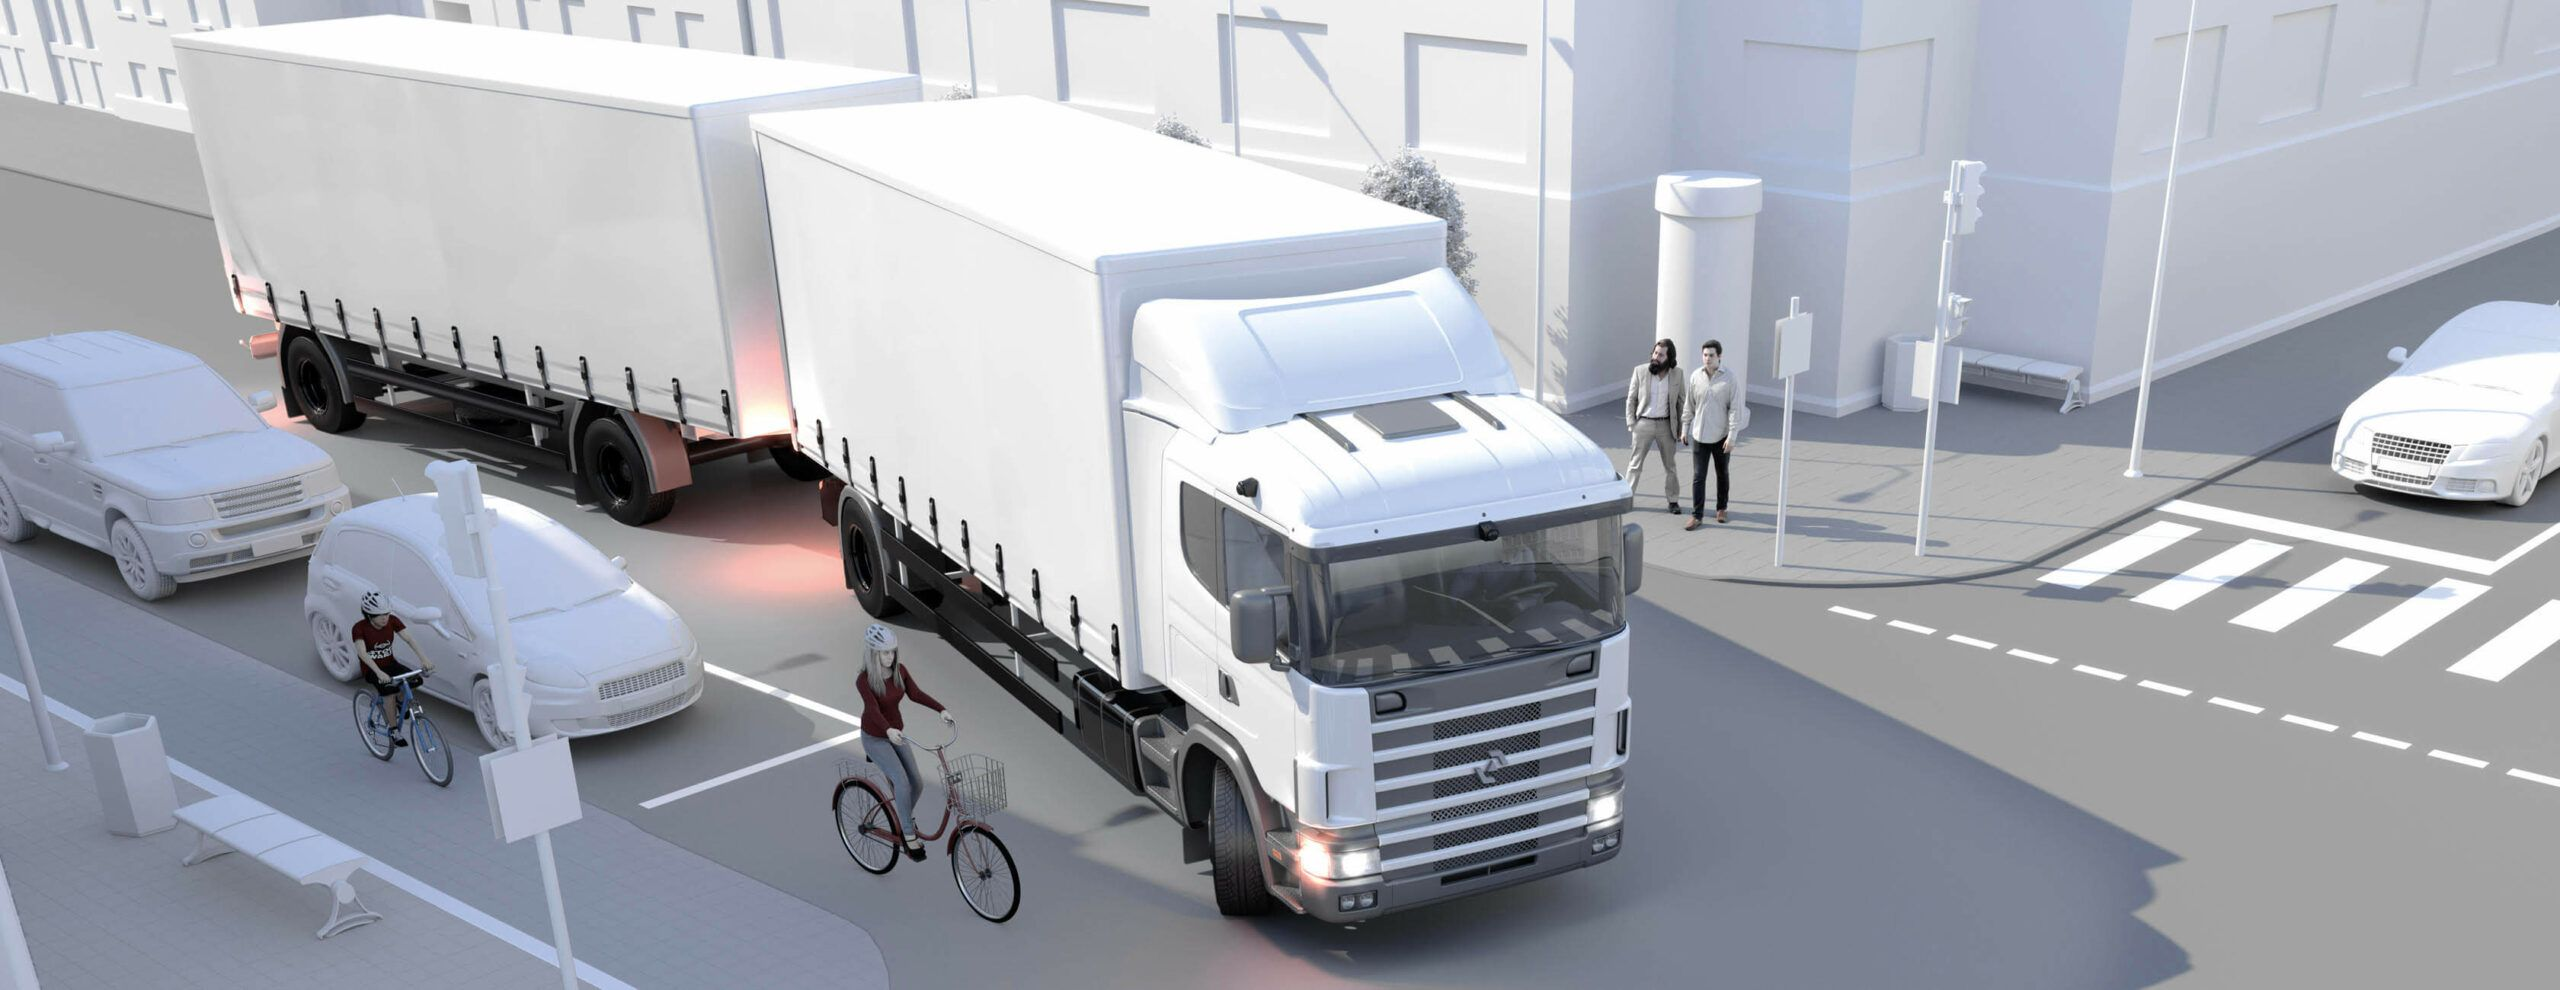
\includegraphics[width=1\linewidth]{images/abbiegeassistent-scaled-7b2478b8}\\[1ex]
    \centering
    \caption{Beispiel Rechtsabbiegen LKW}
    \label{ABBILDUNG}
\end{figure}


Eine besonders bedeutende Neuerung im Bereich der \acf{LKW}-Sicherheit stellen Abbiegeassistenten dar. 
Diese Systeme helfen, den toten Winkel zu reduzieren und somit Unfälle – insbesondere beim Rechtsabbiegen – zu vermeiden. 
Trotz dieser technischen Fortschritte besteht weiterhin Potenzial für weitere Verbesserungen. Eine umfassende Forschung und Entwicklung 
im Bereich von Fahrerassistenzsystemen könnte zukünftig dazu beitragen, das allgemeine Verkehrsrisiko weiter zu senken und die Verkehrssicherheit
signifikant zu erhöhen. [1]

\clearpage

\subsection{Zielsetzung}
Zielsetzung dieser Studienarbeit ist es, einen 
leistungsfähigen Datenlogger zu entwickeln und die Visualisierung 
zu verbessern, um die Funktionalität des Fahrerassistenzsystems zu erhöhen 
und dadurch dessen Entwicklung zu erleichtern. Durch die Implementierung eines 
leistungsfähigen Datenloggers sollen Messwerte systematisch und zuverlässig 
erfasst werden können, was eine effektivere Zusammenarbeit im Entwicklungsteam 
ermöglicht und die Notwendigkeit einer dauerhaften Hardwareverbindung reduziert. Die Optimierung der Visualisierung 
dient dazu, Messergebnisse klarer und übersichtlicher darzustellen, um künftige Analysen und Tests zu vereinfachen und somit
 die Qualität und Genauigkeit der Positionsbestimmung zu erhöhen. Diese Verbesserungen sollen letztlich zu einer höheren Effizienz
  im Entwicklungsprozess führen und 
somit einen wesentlichen Beitrag zur Erhöhung der Verkehrssicherheit leisten.

\clearpage

\section{Rückblick auf das mobile Warnsystem}
\subsection{Konzept und Zielsetzung}
Die vorherige Studienarbeit verfolgte das Ziel, ein mobiles Warnsystem zur Minimierung von 
Abbiegeunfällen zwischen \ac{LKW} und ungeschützten Verkehrsteilnehmenden wie Fußgängerinnen und Radfahrerinnen zu entwickeln.
Zentrales Element dieses Systems war eine mobile Applikation, die als aktiver Bluetooth-Sender fungieren sollte. In Kombination 
mit einem am \ac{LKW} montierten Empfängerboard (basierend auf dem u-blox XPLR-AOA-1 Kit) sollte mithilfe der \acf{AoA}-Technologie 
die Position des Smartphones lokalisiert und bei drohender Gefahr eine Warnung ausgegeben werden. Das System versprach einen 
kostengünstigen und einfach zugänglichen Ansatz zur Verbesserung der Verkehrssicherheit im städtischen Raum.

\subsection{Bluetooth AoA und technische Grundlagen}
Die \ac{AoA}-Technologie ist Teil des Bluetooth 5.1 Standards und ermöglicht die Positionsbestimmung
 eines Senders durch Messung des Einfallswinkels der Funksignale an mehreren Antennen eines Empfängers. 
 Voraussetzung hierfür ist jedoch ein exakter Zugang zu den Bluetooth-Sendeparametern sowie eine Antennenkonfiguration 
 mit bekannten geometrischen Abständen. Das u-blox XPLR-AOA-1 Explorer Kit stellt hierzu eine geeignete Hardwarelösung dar, 
 da es mit einem \ac{AoA}-fähigen Empfängerboard und einem sogenannten Tag (Sender) ausgestattet ist. Ziel der Arbeit war es, das Smartphone 
 funktional durch diesen Tag zu ersetzen. [1][2][3]

 \begin{figure}[H]
    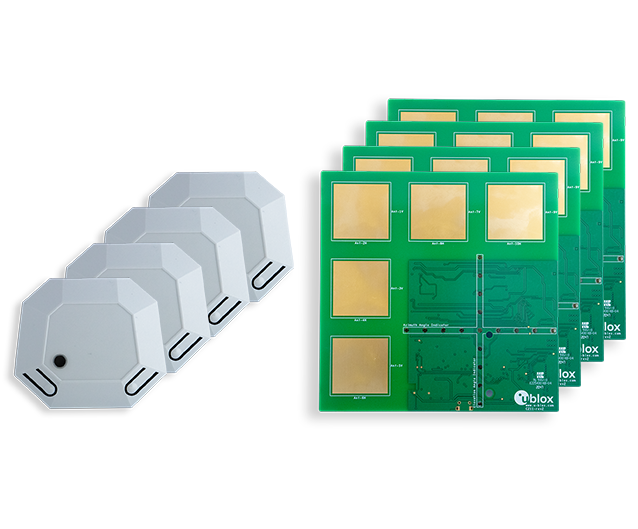
\includegraphics[width=1\linewidth]{images/XPLR-AOA-with-C209-and-C211-02_0}\\[1ex]
    \centering
    \caption{XPLR-AOA Explorer Kit}
    \label{ABBILDUNG}
\end{figure}

 \subsection{Herausforderungen und Gründe für die Projektpause}
 Im praktischen Verlauf der Umsetzung traten mehrere schwerwiegende technische Limitierungen auf, die die Fortführung des Projekts verhinderten:

 \begin{itemize}
    \item Aktuelle Smartphone-Firmware (insbesondere auf Android-Basis) verhindert in der Regel den vollständigen Zugriff auf die Bluetooth-Sendeparameter. Ein gezieltes Emittieren von \acf{BLE}-Signalen, wie es zur \ac{AoA}-Ortung erforderlich ist, ist mit Standard-\acf{SDK} nicht möglich.
    \item Nur wenige aktuelle Mobilgeräte unterstützen Bluetooth 5.1 vollständig, was die Reichweite und Genauigkeit der Ortung stark einschränkt.
    \item Die Emulation des u-blox Tags durch das Smartphone scheiterte daher an mangelnden Systemrechten, fehlender Low-Level-\acf{API}-Zugriffe und nicht ausreichender Hardwareunterstützung.
 \end{itemize}
Diese Faktoren führten dazu, dass das Projekt in der geplanten Form nicht abgeschlossen werden konnte. 
Die zugrundeliegende Idee bleibt jedoch vielversprechend und kann in Zukunft wieder aufgegriffen werden, sobald sich 
die technischen Rahmenbedingungen verbessert haben.[4][5][6][7]

\clearpage

\section{Grundlagen Datenlogger}
\subsection{Zweck und Funktionalität eines Datenloggers}
Ein Datenlogger ist ein autonom arbeitendes Gerät oder Softwaremodul, das physikalische oder digitale Messwerte über einen definierten 
Zeitraum hinweg aufzeichnet. Ziel ist es, Veränderungen systematisch und zuverlässig zu erfassen, um sie später analysieren, auswerten 
oder dokumentieren zu können. Typische erfasste Daten umfassen beispielsweise Temperatur, Spannung, Zeitstempel, Lage- oder Positionsdaten.

\begin{figure}[H]
    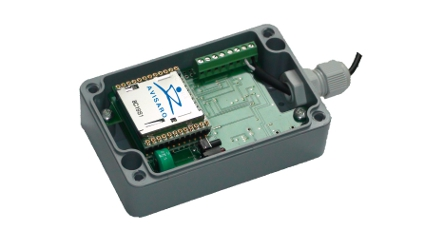
\includegraphics[width=1\linewidth]{images/Datalogger}\\[1ex]
    \centering
    \caption{Datenlogger Cube (Avisaro 2.0) zur Speicherung von Sensor- und Prozessdaten}
    \label{ABBILDUNG}
\end{figure}

Im Gegensatz zu interaktiven Messsystemen arbeitet ein Datenlogger in der Regel unabhängig und ohne dauerhafte Verbindung 
zu einem Steuergerät. Dies macht ihn besonders geeignet für mobile oder schwer zugängliche Anwendungen. Durch kontinuierliche 
Aufzeichnung lassen sich Messwerte nachvollziehbar dokumentieren, was vor allem in der Entwicklung, Fehlersuche und Validierung technischer 
Systeme von Bedeutung ist.

Wichtige Eigenschaften eines Datenloggers sind unter anderem eine ausreichende Speicherkapazität, 
Energieeffizienz und die Kompatibilität zu verschiedenen Datenformaten wie \acf{CSV} oder \acf{JSON}. Moderne Logger 
bieten darüber hinaus Schnittstellen für drahtlose Datenübertragung oder automatisierte Synchronisation mit Analysetools.

\subsection{Anwendungsbereiche im Kontext der Studienarbeit}
Im Rahmen dieser Studienarbeit wird der Datenlogger gezielt eingesetzt, um die Entwicklungsarbeit am Bluetooth-\ac{AoA}-basierten
 Lokalisierungssystem effizienter und flexibler zu gestalten. Ziel ist es, die Abhängigkeit von einer aktiven Verbindung zur 
 Hardware während der Test- und Anpassungsphasen zu minimieren. Personen, die an der Parametrierung oder Feinjustierung des Systems
  arbeiten, sollen in die Lage versetzt werden, auch ohne direkte Verbindung zur u-blox-Hardware auf reale Messdaten zuzugreifen.

Der Datenlogger dient dabei nicht nur der reinen Aufzeichnung, sondern ermöglicht die Speicherung von tatsächlich erfassten, 
originalgetreuen Messwerten. Diese Werte können anschließend in separate Programme oder Auswertungswerkzeuge importiert werden,
 um dort Berechnungen, Analysen und grafische Darstellungen durchzuführen. Änderungen an Parametern oder Auswertealgorithmen können 
 somit auf Basis gespeicherter Daten vorgenommen und getestet werden, ohne dass dafür eine erneute Datenerfassung mit der realen Sensorik notwendig ist.

Darüber hinaus erlaubt der Datenlogger eine „Offline-Simulation“ oder ein Daten-Replay mit echten Werten. Diese Vorgehensweise bietet den 
Vorteil, dass Optimierungen zunächst im Testsystem geprüft werden können. Erst wenn ein Ergebnis zufriedenstellend ist, wird es auf das reale 
System übertragen. Damit leistet der Datenlogger einen wesentlichen Beitrag zur Entkopplung von Entwicklung und Hardwareverfügbarkeit, 
was vor allem in Teamkonstellationen und bei paralleler Arbeit an mehreren Teilaspekten des Systems von großem Nutzen ist.

\subsection{Vorhandene Herausforderungen und Lösungsansätze}
Bei der Entwicklung eines zuverlässigen Datenloggers im Kontext des Bluetooth\ac{AoA}-Systems treten verschiedene Herausforderungen auf. 
Eine der zentralen Schwierigkeiten liegt in der exakten zeitlichen Zuordnung der erfassten Daten. Für eine sinnvolle Auswertung müssen 
Zeitstempel, Empfangswinkel und weitere Messgrößen synchronisiert und konsistent gespeichert werden.

Ein weiteres Problem stellt die effiziente und verlustfreie Speicherung großer Datenmengen dar. 
Hierbei müssen sowohl die Speicherkapazität als auch die Lesbarkeit und Weiterverwendbarkeit berücksichtigt werden. Gerade 
im Hinblick auf die spätere Analyse mit gängigen Tools wie Python oder MATLAB ist ein gut strukturiertes Datenformat – etwa \ac{CSV} oder \ac{JSON} – von 
hoher Bedeutung.

Auch die Integration in bestehende Entwicklungsprozesse erfordert eine durchdachte Schnittstellengestaltung.
 Der Datenlogger muss flexibel und modular aufgebaut sein, damit er problemlos in verschiedene Testumgebungen 
 eingebunden werden kann. Gleichzeitig soll der Energieverbrauch möglichst gering gehalten werden, um auch den mobilen Einsatz über längere
  Zeiträume hinweg zu ermöglichen.

Lösungsansätze bestehen in der Verwendung eines einfachen, standardisierten Speicherformats, einem modularen 
Softwaredesign mit klar dokumentierten Schnittstellen sowie in der Implementierung grundlegender Fehlererkennungs- und Synchronisationsmechanismen. 
Diese Maßnahmen sollen sicherstellen, dass der Datenlogger zuverlässig, energieeffizient und nutzerfreundlich eingesetzt werden kann.

\clearpage

\section{Entwicklung des Datenloggers}
\subsection{Anforderungen an die Software}
Die Software des Datenloggers muss in der Lage sein, Messwerte des Bluetooth-\ac{AoA}-Systems automatisch und kontinuierlich zu erfassen, zu speichern 
und für die spätere Analyse verfügbar zu machen. Zu den grundlegenden funktionalen Anforderungen gehört die Unterstützung strukturierter Exportformate 
wie \ac{CSV} oder \ac{JSON}, um die Weiterverarbeitung in gängigen Tools wie Python oder MATLAB zu ermöglichen. Zudem soll die Software konfigurierbar sein, 
um Messparameter wie Samplingrate oder Filterbedingungen flexibel anpassen zu können.

Nicht-funktionale Anforderungen betreffen insbesondere die Zuverlässigkeit und Ressourcenschonung. Die Anwendung soll auch bei längeren 
Aufzeichnungen stabil laufen, sparsam mit Speicher und Energie umgehen und eine einfache Bedienbarkeit bieten. Eine modulare Architektur ist dabei 
essenziell, um Erweiterungen oder Anpassungen effizient umzusetzen.

Für das vorliegende Projekt ist außerdem besonders wichtig, dass die Software auch ohne direkte Verbindung zur u-blox-Hardware 
einsatzfähig ist. Aufgezeichnete Daten müssen für eine Offline-Auswertung und Visualisierung nutzbar sein, um iterative Verbesserungen an 
Parametern oder Algorithmen unabhängig von der Hardwareumgebung vornehmen zu können.

\subsection{Auswahl geeigneter Technologien und Tools}
\subsection{Implementierung und Integration in bestehende Systeme}
\subsection{Ergebnisse und Evaluation}

\section{Grundlagen der Visualisierung}
\subsection{Anforderungen an eine effektive Visualisierung}
\subsection{Darstellungsmöglichkeiten und -technologien}

\section{Entwicklung der neuen Visualisierung}
\subsection{Analyse der bestehenden Visualisierung}
\subsection{Konzept einer verbesserten Visualisierung}
\subsection{Implementierung der verbesserten Visualisierung}
\subsection{Ergebnisse und Benutzerfreundlichkeit}

\section{Test und Validierung}
\subsection{Testmethodik und -umgebung}
\subsection{Ergebnisse der Tests}
\subsection{Diskussion der Testergebnisse und Optimierungspotentiale}

\section{Kritische Bewertung und Ausblick}
\subsection{Reflexion der erreichten Ergebnisse}
\subsection{Grenzen der aktuellen Umsetzung}
\subsection{Vorschläge für zukünftige Weiterentwicklungen}


\clearpage
%---------------------------------------------------------
% Bibliografie
%---------------------------------------------------------
\begingroup
\renewcommand{\bibfont}{\fontsize{13pt}{12pt}\selectfont}  
\sloppy
\nocite{*}
\printbibliography
\endgroup

\end{document}
